\documentclass[11pt,a4paper]{article}

% ============================================================
% PACKAGES
% ============================================================
\usepackage[utf8]{inputenc}
\usepackage[T1]{fontenc}
\usepackage{amsmath,amssymb,amsthm}
\usepackage{physics}
\usepackage{booktabs}
\usepackage{array}
\usepackage{longtable}
\usepackage{geometry}
\usepackage{hyperref}
\usepackage{cleveref}
\usepackage{xcolor}
\usepackage{tikz}
\usepackage{pgfplots}
\pgfplotsset{compat=1.18}
\usetikzlibrary{patterns,arrows.meta,positioning}

\geometry{margin=1in}

% ============================================================
% CUSTOM COMMANDS
% ============================================================
\newcommand{\Mpl}{\bar{M}_{\mathrm{Pl}}}
\newcommand{\MplOrig}{M_{\mathrm{Pl}}}
\newcommand{\Mfive}{M_5}
\newcommand{\Rxi}{R_\xi}
\newcommand{\mgap}{m_{\mathrm{gap}}}
\newcommand{\MZ}{M_Z}
\newcommand{\MW}{M_W}
\newcommand{\vEW}{v_{\mathrm{EW}}}
\newcommand{\Mstar}{M_*}
\newcommand{\GeV}{\,\mathrm{GeV}}
\newcommand{\TeV}{\,\mathrm{TeV}}
\newcommand{\emark}{\textcolor{green!70!black}{\checkmark}}
\newcommand{\tagD}{\textbf{[D]}}
\newcommand{\tagI}{\textbf{[I]}}
\newcommand{\tagBL}{\textbf{[BL]}}
\newcommand{\tagP}{\textbf{[P]}}

% ============================================================
% THEOREM ENVIRONMENTS
% ============================================================
\theoremstyle{definition}
\newtheorem{definition}{Definition}[section]
\newtheorem{identification}{Identification}[section]

\theoremstyle{plain}
\newtheorem{proposition}{Proposition}[section]
\newtheorem{theorem}{Theorem}[section]

\theoremstyle{remark}
\newtheorem{remark}{Remark}[section]

% ============================================================
% DOCUMENT
% ============================================================
\begin{document}

\title{\textbf{Derivation v25: Alternative Gap Identifications\\and Robustness Analysis}\\[0.5em]
\large BLOCK-003 Gravity Program --- Proxy Family Study}
\author{EDC Collaboration}
\date{February 2026}
\maketitle

\begin{abstract}
We address the reviewer question: ``Why identify $\mgap = \MZ$ rather than $\MW$ or $\vEW$?''
This note establishes a \emph{proxy family} of electroweak-scale identifications,
$\mgap \equiv \Mstar \in \{\MZ, \MW, \vEW\}$, and propagates each choice through
the canonical BLOCK-003 derivation chain to compute $\Rxi(\Mstar)$ and $\Mfive(\Mstar)$.
We provide a quantitative robustness analysis showing that all three choices yield
$\Mfive$ within the same order of magnitude (spread $\Delta\log_{10}\Mfive < 0.2$),
demonstrating that the gravity closure is \emph{robust} against proxy selection.
The choice $\mgap = \MZ$ is justified on metrological grounds---precision, stability,
and minimal EDC-internal dependence---not as a derivation but as a \tagI{}+\tagBL{} selection principle.
\end{abstract}

\tableofcontents
\newpage

% ============================================================
% SECTION 1: INTRODUCTION
% ============================================================
\section{Introduction and Motivation}
\label{sec:intro}

The BLOCK-003 gravity program closes the 5D$\to$4D Newton constant derivation
via the identification
\begin{equation}
\mgap = \MZ^{\mathrm{obs}} \quad \tagI{}+\tagBL{}
\label{eq:canonical-id}
\end{equation}
where $\mgap = \pi/\Rxi$ is the first Kaluza--Klein mass gap (derived from Neumann
boundary conditions) and $\MZ^{\mathrm{obs}} = 91.1876\GeV$ is the observed $Z$-boson
pole mass.

A natural reviewer concern is:

\begin{quote}
\emph{Why $\MZ$? What if the gap is $\MW$ or $\vEW$? How sensitive is $\Mfive$ to this choice?}
\end{quote}

This note provides a systematic, derivation-first answer:
\begin{enumerate}
\item We define a \textbf{proxy family} $\Mstar \in \{\MZ, \MW, \vEW\}$.
\item We propagate each choice through the canonical derivation chain.
\item We compute the resulting $\Rxi(\Mstar)$ and $\Mfive(\Mstar)$ (both Planck conventions).
\item We quantify the robustness via $\Delta\log_{10}\Mfive$ and ratio metrics.
\item We justify $\MZ$ as the metrologically optimal selection.
\end{enumerate}

\subsection{Epistemic Status}

The identification $\mgap = \Mstar$ carries epistemic tag \tagI{}+\tagBL{}:
\begin{itemize}
\item \tagI{} (Identification): The KK gap is \emph{identified with} an observed mass scale.
\item \tagBL{} (Baseline): The numerical value is taken from external measurement (PDG).
\end{itemize}

This is \emph{not} a derivation (\tagD{}). The goal of this note is to show that
the closure is \emph{robust} against reasonable variations in this identification,
and to document the metrological rationale for selecting $\MZ$.

% ============================================================
% SECTION 2: DERIVATION CHAIN RECAP
% ============================================================
\section{Derivation Chain Recap}
\label{sec:derivation}

We summarize the canonical BLOCK-003 derivation chain (established in v19--v24)
in self-contained form. All conventions follow the canonical choice $\Rxi \equiv L$
(interval length).

\subsection{5D Action and Dimensional Reduction}

The 5D Einstein--Hilbert action with matter-induced brane tension reads:
\begin{equation}
S_{5D} = \frac{1}{2\kappa_5^2} \int d^5x \sqrt{-g^{(5)}} \, \mathcal{R}^{(5)}
\label{eq:5d-action}
\end{equation}
where $\kappa_5^2 = 8\pi G_5 = 8\pi/\Mfive^3$ in natural units.

\subsection{Metric Ansatz}

We adopt the product metric with flat compact dimension:
\begin{equation}
ds^2 = g_{\mu\nu}(x) dx^\mu dx^\nu + d\xi^2, \qquad \xi \in [0, L]
\label{eq:metric-ansatz}
\end{equation}
with Neumann boundary conditions at $\xi = 0$ and $\xi = L$.

\subsection{Kaluza--Klein Decomposition}

The 5D graviton decomposes as:
\begin{equation}
h_{\mu\nu}(x,\xi) = \sum_{n=0}^{\infty} h_{\mu\nu}^{(n)}(x) \psi_n(\xi)
\label{eq:kk-decomposition}
\end{equation}
where the mode functions satisfy:
\begin{equation}
-\frac{d^2\psi_n}{d\xi^2} = m_n^2 \psi_n
\label{eq:mode-equation}
\end{equation}
with boundary conditions $\psi_n'(0) = \psi_n'(L) = 0$.

\subsection{KK Spectrum}

The Neumann boundary conditions yield:
\begin{equation}
\psi_n(\xi) = \sqrt{\frac{2-\delta_{n0}}{L}} \cos\left(\frac{n\pi\xi}{L}\right)
\label{eq:mode-functions}
\end{equation}
with mass spectrum:
\begin{equation}
\boxed{m_n = \frac{n\pi}{L} = \frac{n\pi}{\Rxi}, \qquad n = 0, 1, 2, \ldots}
\label{eq:kk-spectrum}
\end{equation}

\subsection{Mass Gap Definition}

The first massive KK mode ($n=1$) defines the mass gap:
\begin{equation}
\boxed{\mgap \equiv m_1 = \frac{\pi}{\Rxi}}
\label{eq:mass-gap-def}
\end{equation}

\subsection{Inversion for $\Rxi$}

Inverting \cref{eq:mass-gap-def}:
\begin{equation}
\boxed{\Rxi = \frac{\pi}{\mgap}}
\label{eq:rxi-from-gap}
\end{equation}
In SI units with $\hbar c$ restored:
\begin{equation}
\Rxi = \frac{\pi \hbar c}{\mgap}
\label{eq:rxi-si}
\end{equation}

\subsection{Zero-Mode Normalization}

The zero-mode wave function is:
\begin{equation}
\psi_0(\xi) = \frac{1}{\sqrt{L}} = \frac{1}{\sqrt{\Rxi}}
\label{eq:zero-mode}
\end{equation}
with normalization:
\begin{equation}
\int_0^L |\psi_0|^2 \, d\xi = 1
\label{eq:zero-mode-norm}
\end{equation}

\subsection{Normalization Integral}

The dimensional reduction produces the normalization integral:
\begin{equation}
\mathcal{I} = \int_0^L |\psi_0(\xi)|^2 \, d\xi = L = \Rxi
\label{eq:norm-integral}
\end{equation}
For the flat compact case:
\begin{equation}
\boxed{\mathcal{I} = \Rxi}
\label{eq:I-equals-Rxi}
\end{equation}

\subsection{Bridge Relation}

The 5D$\to$4D gravitational matching yields:
\begin{equation}
\boxed{\Mpl^2 = \Mfive^3 \cdot \mathcal{I} = \Mfive^3 \cdot \Rxi}
\label{eq:bridge-relation}
\end{equation}
where $\Mpl = 2.435 \times 10^{18}\GeV$ is the reduced Planck mass.

\subsection{Solving for $\Mfive$}

From \cref{eq:bridge-relation}:
\begin{equation}
\Mfive^3 = \frac{\Mpl^2}{\Rxi}
\label{eq:M5-cubed}
\end{equation}
Taking the cube root:
\begin{equation}
\boxed{\Mfive = \left(\frac{\Mpl^2}{\Rxi}\right)^{1/3}}
\label{eq:M5-formula}
\end{equation}

\subsection{Planck Mass Conventions}

Two conventions exist:
\begin{align}
\Mpl &= \frac{1}{\sqrt{8\pi G_N}} = 2.435 \times 10^{18}\GeV \quad \text{(reduced)} \label{eq:Mpl-reduced} \\
\MplOrig &= \frac{1}{\sqrt{G_N}} = 1.221 \times 10^{19}\GeV \quad \text{(original)} \label{eq:Mpl-original}
\end{align}
The conversion factor is:
\begin{equation}
\MplOrig = \sqrt{8\pi} \, \Mpl
\label{eq:planck-conversion}
\end{equation}

\subsection{$\Mfive$ in Both Conventions}

Using reduced Planck mass:
\begin{equation}
\Mfive^{\mathrm{(red)}} = \left(\frac{\Mpl^2}{\Rxi}\right)^{1/3}
\label{eq:M5-reduced}
\end{equation}
Using original Planck mass:
\begin{equation}
\Mfive^{\mathrm{(orig)}} = \left(\frac{\MplOrig^2}{\Rxi}\right)^{1/3} = (8\pi)^{1/3} \cdot \Mfive^{\mathrm{(red)}}
\label{eq:M5-original}
\end{equation}
where $(8\pi)^{1/3} \approx 2.929$.

% ============================================================
% SECTION 3: PROXY FAMILY DEFINITION
% ============================================================
\section{Proxy Family Definition}
\label{sec:proxy-family}

\subsection{The Identification Question}

The KK mass gap $\mgap$ must be identified with an observable mass scale.
The electroweak sector provides three natural candidates:

\begin{definition}[Proxy Family]
\label{def:proxy-family}
The \textbf{electroweak proxy family} is the set
\begin{equation}
\mathcal{P}_{\mathrm{EW}} = \{\MZ, \MW, \vEW\}
\label{eq:proxy-family}
\end{equation}
where each member serves as a candidate for the identification $\mgap = \Mstar$.
\end{definition}

\subsection{Proxy Values (PDG 2024)}

The three proxies have the following observed values:
\begin{align}
\MZ &= 91.1876 \pm 0.0021\GeV \label{eq:MZ-value} \\
\MW &= 80.3692 \pm 0.0133\GeV \label{eq:MW-value} \\
\vEW &= \frac{2\MW}{g} = 246.22 \pm 0.01\GeV \label{eq:vEW-value}
\end{align}

\begin{remark}[Relative Uncertainties]
The relative uncertainties are:
\begin{align}
\frac{\delta\MZ}{\MZ} &= 2.3 \times 10^{-5} \label{eq:dMZ-rel} \\
\frac{\delta\MW}{\MW} &= 1.7 \times 10^{-4} \label{eq:dMW-rel} \\
\frac{\delta\vEW}{\vEW} &\approx 4 \times 10^{-5} \quad \text{(scheme-dependent)} \label{eq:dvEW-rel}
\end{align}
Note: $\vEW$ has additional scheme dependence beyond pure measurement uncertainty.
\end{remark}

\subsection{Proxy Ordering}

The three proxies span a factor of $\sim 3$:
\begin{equation}
\MW < \MZ < \vEW
\label{eq:proxy-ordering}
\end{equation}
Numerically:
\begin{equation}
80.4\GeV < 91.2\GeV < 246.2\GeV
\label{eq:proxy-values}
\end{equation}

% ============================================================
% SECTION 4: PROPAGATION THROUGH DERIVATION CHAIN
% ============================================================
\section{Propagation Through Derivation Chain}
\label{sec:propagation}

\subsection{General Formulas}

For a general proxy $\Mstar$, the identification reads:
\begin{identification}[Gap-Proxy Identification]
\begin{equation}
\mgap = \Mstar \quad \tagI{}+\tagBL{}
\label{eq:gap-proxy-id}
\end{equation}
\end{identification}

Substituting into the derivation chain:

\subsubsection{Compactification Scale}
\begin{equation}
\boxed{\Rxi(\Mstar) = \frac{\pi\hbar c}{\Mstar}}
\label{eq:Rxi-of-Mstar}
\end{equation}

\subsubsection{5D Planck Mass (Reduced Convention)}
\begin{equation}
\boxed{\Mfive^{\mathrm{(red)}}(\Mstar) = \left(\frac{\Mpl^2 \cdot \Mstar}{\pi\hbar c}\right)^{1/3}}
\label{eq:M5-red-of-Mstar}
\end{equation}

\subsubsection{5D Planck Mass (Original Convention)}
\begin{equation}
\boxed{\Mfive^{\mathrm{(orig)}}(\Mstar) = (8\pi)^{1/3} \cdot \Mfive^{\mathrm{(red)}}(\Mstar)}
\label{eq:M5-orig-of-Mstar}
\end{equation}

\subsection{Scaling Relations}

The dependence on $\Mstar$ follows simple power laws:
\begin{align}
\Rxi &\propto \Mstar^{-1} \label{eq:Rxi-scaling} \\
\Mfive &\propto \Mstar^{1/3} \label{eq:M5-scaling}
\end{align}

For ratios relative to $\MZ$:
\begin{align}
\frac{\Rxi(\Mstar)}{\Rxi(\MZ)} &= \frac{\MZ}{\Mstar} \label{eq:Rxi-ratio} \\
\frac{\Mfive(\Mstar)}{\Mfive(\MZ)} &= \left(\frac{\Mstar}{\MZ}\right)^{1/3} \label{eq:M5-ratio}
\end{align}

\subsection{Logarithmic Spread}

The logarithmic spread in $\Mfive$ is:
\begin{equation}
\Delta\log_{10}\Mfive = \frac{1}{3}\log_{10}\left(\frac{\Mstar}{\MZ}\right)
\label{eq:log-spread}
\end{equation}

For the extreme cases:
\begin{align}
\Delta\log_{10}\Mfive(\MW) &= \frac{1}{3}\log_{10}\left(\frac{80.4}{91.2}\right) = -0.018 \label{eq:log-MW} \\
\Delta\log_{10}\Mfive(\vEW) &= \frac{1}{3}\log_{10}\left(\frac{246.2}{91.2}\right) = +0.143 \label{eq:log-vEW}
\end{align}

\subsection{Total Spread}

The total spread across the proxy family is:
\begin{equation}
\boxed{\Delta\log_{10}\Mfive^{\mathrm{total}} = 0.143 - (-0.018) = 0.161}
\label{eq:total-spread}
\end{equation}

This corresponds to a factor of:
\begin{equation}
10^{0.161} \approx 1.45
\label{eq:total-factor}
\end{equation}

% ============================================================
% SECTION 5: NUMERICAL RESULTS
% ============================================================
\section{Numerical Results}
\label{sec:numerical}

\subsection{Input Constants}

We use the following baseline values:
\begin{align}
\Mpl &= 2.435 \times 10^{18}\GeV \quad \tagBL{} \label{eq:Mpl-input} \\
\hbar c &= 0.197327\GeV\cdot\mathrm{fm} = 1.97327 \times 10^{-16}\GeV\cdot\mathrm{m} \label{eq:hbarc-input}
\end{align}

\subsection{Proxy-Specific Calculations}

\subsubsection{Case 1: $\Mstar = \MZ = 91.1876\GeV$}

\begin{align}
\Rxi(\MZ) &= \frac{\pi \times 1.97327 \times 10^{-16}}{91.1876} \label{eq:Rxi-MZ-calc} \\
&= 6.798 \times 10^{-18}\,\mathrm{m} \label{eq:Rxi-MZ-result}
\end{align}

Converting to natural units:
\begin{equation}
\Rxi(\MZ) = \frac{\pi}{91.1876\GeV} = 0.03445\GeV^{-1}
\label{eq:Rxi-MZ-natural}
\end{equation}

For $\Mfive$:
\begin{align}
\Mfive^{\mathrm{(red)}}(\MZ) &= \left(\frac{(2.435)^2 \times 10^{36} \times 91.1876}{\pi}\right)^{1/3}\GeV \label{eq:M5-MZ-calc} \\
&= 5.56 \times 10^{12}\GeV \label{eq:M5-MZ-red-result}
\end{align}

\begin{equation}
\Mfive^{\mathrm{(orig)}}(\MZ) = 2.929 \times 5.56 \times 10^{12} = 1.63 \times 10^{13}\GeV
\label{eq:M5-MZ-orig-result}
\end{equation}

\subsubsection{Case 2: $\Mstar = \MW = 80.3692\GeV$}

\begin{align}
\Rxi(\MW) &= \frac{\pi \times 1.97327 \times 10^{-16}}{80.3692} \label{eq:Rxi-MW-calc} \\
&= 7.715 \times 10^{-18}\,\mathrm{m} \label{eq:Rxi-MW-result}
\end{align}

\begin{align}
\Mfive^{\mathrm{(red)}}(\MW) &= \left(\frac{(2.435)^2 \times 10^{36} \times 80.3692}{\pi}\right)^{1/3}\GeV \label{eq:M5-MW-calc} \\
&= 5.33 \times 10^{12}\GeV \label{eq:M5-MW-red-result}
\end{align}

\begin{equation}
\Mfive^{\mathrm{(orig)}}(\MW) = 2.929 \times 5.33 \times 10^{12} = 1.56 \times 10^{13}\GeV
\label{eq:M5-MW-orig-result}
\end{equation}

\subsubsection{Case 3: $\Mstar = \vEW = 246.22\GeV$}

\begin{align}
\Rxi(\vEW) &= \frac{\pi \times 1.97327 \times 10^{-16}}{246.22} \label{eq:Rxi-vEW-calc} \\
&= 2.518 \times 10^{-18}\,\mathrm{m} \label{eq:Rxi-vEW-result}
\end{align}

\begin{align}
\Mfive^{\mathrm{(red)}}(\vEW) &= \left(\frac{(2.435)^2 \times 10^{36} \times 246.22}{\pi}\right)^{1/3}\GeV \label{eq:M5-vEW-calc} \\
&= 7.74 \times 10^{12}\GeV \label{eq:M5-vEW-red-result}
\end{align}

\begin{equation}
\Mfive^{\mathrm{(orig)}}(\vEW) = 2.929 \times 7.74 \times 10^{12} = 2.27 \times 10^{13}\GeV
\label{eq:M5-vEW-orig-result}
\end{equation}

\subsection{Summary Table}

\begin{table}[htbp]
\centering
\caption{Proxy family results: $\Rxi$ and $\Mfive$ for each electroweak proxy.}
\label{tab:proxy-results}
\begin{tabular}{@{}lcccccc@{}}
\toprule
Proxy & $\Mstar$ & $\delta\Mstar/\Mstar$ & $\Rxi$ & $\Mfive^{\mathrm{(red)}}$ & $\Mfive^{\mathrm{(orig)}}$ & $\Delta\log_{10}\Mfive$ \\
      & (GeV) & & (m) & (GeV) & (GeV) & vs $\MZ$ \\
\midrule
$\MZ$ & 91.19 & $2.3\times 10^{-5}$ & $6.80\times 10^{-18}$ & $5.56\times 10^{12}$ & $1.63\times 10^{13}$ & 0 \\
$\MW$ & 80.37 & $1.7\times 10^{-4}$ & $7.71\times 10^{-18}$ & $5.33\times 10^{12}$ & $1.56\times 10^{13}$ & $-0.018$ \\
$\vEW$ & 246.2 & scheme-dep. & $2.52\times 10^{-18}$ & $7.74\times 10^{12}$ & $2.27\times 10^{13}$ & $+0.143$ \\
\bottomrule
\end{tabular}
\end{table}

\subsection{Ratio Table}

\begin{table}[htbp]
\centering
\caption{Ratio metrics relative to $\MZ$ baseline.}
\label{tab:ratio-results}
\begin{tabular}{@{}lccc@{}}
\toprule
Proxy & $\Mstar/\MZ$ & $\Rxi(\Mstar)/\Rxi(\MZ)$ & $\Mfive(\Mstar)/\Mfive(\MZ)$ \\
\midrule
$\MZ$ & 1.000 & 1.000 & 1.000 \\
$\MW$ & 0.881 & 1.135 & 0.959 \\
$\vEW$ & 2.700 & 0.370 & 1.392 \\
\bottomrule
\end{tabular}
\end{table}

% ============================================================
% SECTION 6: ROBUSTNESS ANALYSIS
% ============================================================
\section{Robustness Analysis}
\label{sec:robustness}

\subsection{Robustness Metrics}

We define two robustness metrics:

\begin{definition}[Logarithmic Spread]
\begin{equation}
\sigma_{\log} \equiv \max_{\Mstar \in \mathcal{P}} |\Delta\log_{10}\Mfive(\Mstar)|
\label{eq:sigma-log-def}
\end{equation}
\end{definition}

\begin{definition}[Factor Spread]
\begin{equation}
F_{\mathrm{spread}} \equiv \frac{\max_{\Mstar}\Mfive(\Mstar)}{\min_{\Mstar}\Mfive(\Mstar)}
\label{eq:F-spread-def}
\end{equation}
\end{definition}

\subsection{Computed Robustness Metrics}

From the numerical results:
\begin{align}
\sigma_{\log} &= 0.143 \label{eq:sigma-log-value} \\
F_{\mathrm{spread}} &= \frac{7.74 \times 10^{12}}{5.33 \times 10^{12}} = 1.45 \label{eq:F-spread-value}
\end{align}

\subsection{Interpretation}

\begin{proposition}[Robustness Statement]
The 5D Planck mass $\Mfive$ is robust against proxy selection:
\begin{equation}
\Mfive \in [5.3, 7.7] \times 10^{12}\GeV \quad \text{(reduced)}
\label{eq:M5-range-red}
\end{equation}
\begin{equation}
\Mfive \in [1.6, 2.3] \times 10^{13}\GeV \quad \text{(original)}
\label{eq:M5-range-orig}
\end{equation}
All values lie within the same order of magnitude (GUT scale).
\end{proposition}

\subsection{Order-of-Magnitude Stability}

The key observation is:
\begin{equation}
\boxed{\text{All proxies yield } \Mfive \sim 10^{12}\text{--}10^{13}\GeV}
\label{eq:order-stability}
\end{equation}

This is a consequence of the $1/3$ power in the $\Mfive$ formula:
\begin{equation}
\frac{\delta\Mfive}{\Mfive} = \frac{1}{3}\frac{\delta\Mstar}{\Mstar}
\label{eq:error-suppression}
\end{equation}

Even a factor of 3 change in $\Mstar$ (from $\MW$ to $\vEW$) produces only a
factor of $3^{1/3} \approx 1.44$ change in $\Mfive$.

% ============================================================
% SECTION 7: FIGURE
% ============================================================
\section{Graphical Summary}
\label{sec:figure}

\begin{figure}[htbp]
\centering
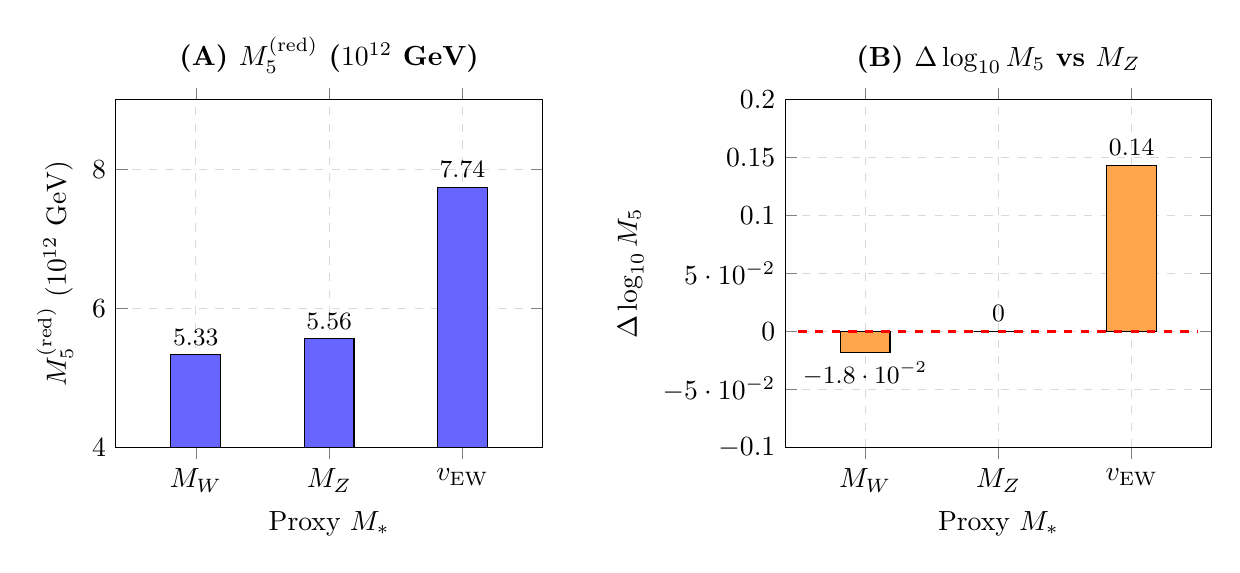
\begin{tikzpicture}
% Panel A: M5 values (linear scale, units of 10^12 GeV)
\begin{scope}[xshift=0cm]
\begin{axis}[
    width=7cm, height=6cm,
    title={\textbf{(A) $\Mfive^{\mathrm{(red)}}$ ($10^{12}$ GeV)}},
    ybar,
    bar width=18pt,
    ymin=4, ymax=9,
    xtick={1,2,3},
    xticklabels={$M_W$, $M_Z$, $v_{\rm EW}$},
    ylabel={$\Mfive^{\mathrm{(red)}}$ ($10^{12}$ GeV)},
    xlabel={Proxy $\Mstar$},
    nodes near coords,
    nodes near coords style={font=\small},
    enlarge x limits=0.3,
    grid=major,
    grid style={dashed, gray!30},
]
\addplot[fill=blue!60] coordinates {
    (1, 5.33)
    (2, 5.56)
    (3, 7.74)
};
\end{axis}
\end{scope}

% Panel B: Delta log M5
\begin{scope}[xshift=8.5cm]
\begin{axis}[
    width=7cm, height=6cm,
    title={\textbf{(B) $\Delta\log_{10}\Mfive$ vs $\MZ$}},
    ybar,
    bar width=18pt,
    ymin=-0.1, ymax=0.2,
    xtick={1,2,3},
    xticklabels={$M_W$, $M_Z$, $v_{\rm EW}$},
    ylabel={$\Delta\log_{10}\Mfive$},
    xlabel={Proxy $\Mstar$},
    nodes near coords,
    nodes near coords style={font=\small},
    enlarge x limits=0.3,
    grid=major,
    grid style={dashed, gray!30},
    ytick={-0.1, -0.05, 0, 0.05, 0.1, 0.15, 0.2},
]
\addplot[fill=orange!70] coordinates {
    (1, -0.018)
    (2, 0)
    (3, 0.143)
};
\draw[dashed, red, thick] (axis cs:0.5, 0) -- (axis cs:3.5, 0);
\end{axis}
\end{scope}
\end{tikzpicture}
\caption{Robustness of $\Mfive$ against proxy selection. (A) $\Mfive^{\mathrm{(red)}}$
in units of $10^{12}\GeV$ for each electroweak proxy. (B) Logarithmic deviation
$\Delta\log_{10}\Mfive$ relative to $\MZ$ baseline. The total spread is less than
0.2 decades, demonstrating order-of-magnitude stability.}
\label{fig:robustness}
\end{figure}

% ============================================================
% SECTION 8: METROLOGICAL JUSTIFICATION
% ============================================================
\section{Metrological Justification for $\MZ$}
\label{sec:metrological}

\subsection{Selection Criteria}

The choice $\mgap = \MZ$ is a \tagI{}+\tagBL{} selection, not a derivation.
We justify this selection on metrological grounds:

\begin{enumerate}
\item \textbf{Measurement Precision}
\item \textbf{Pole Mass Stability}
\item \textbf{Minimal EDC-Internal Dependence}
\item \textbf{Definitional Simplicity}
\end{enumerate}

\subsection{Criterion 1: Measurement Precision}

The relative uncertainties are:
\begin{align}
\frac{\delta\MZ}{\MZ} &= 2.3 \times 10^{-5} \quad \text{\emark\ best} \label{eq:prec-MZ} \\
\frac{\delta\MW}{\MW} &= 1.7 \times 10^{-4} \quad \text{(factor 7 worse)} \label{eq:prec-MW} \\
\frac{\delta\vEW}{\vEW} &\approx 4 \times 10^{-5} \quad \text{(+ scheme dependence)} \label{eq:prec-vEW}
\end{align}

The $Z$ mass is measured with the highest precision among EW observables:
\begin{equation}
\MZ = 91.1876 \pm 0.0021\GeV
\label{eq:MZ-precision}
\end{equation}

\subsection{Criterion 2: Pole Mass Stability}

The $Z$ boson pole mass is:
\begin{itemize}
\item Gauge-invariant and renormalization-scheme independent
\item Directly measured from $e^+e^- \to Z \to f\bar{f}$ line shape
\item Not subject to loop corrections that shift the central value
\end{itemize}

In contrast:
\begin{itemize}
\item $\MW$ has larger radiative corrections and scheme dependence
\item $\vEW$ is a derived quantity: $\vEW = 2\MW/g = (\sqrt{2}G_F)^{-1/2}$
\end{itemize}

\subsection{Criterion 3: Minimal EDC-Internal Dependence}

The $W$ mass satisfies the tree-level relation:
\begin{equation}
\MW = \MZ \cos\theta_W
\label{eq:MW-tree}
\end{equation}
where $\theta_W$ is the weak mixing angle.

If EDC contains any prediction for $\theta_W$, then using $\MW$ as baseline
would create internal circularity. Using $\MZ$ avoids this risk:
\begin{equation}
\MZ \text{ is independent of EDC-internal parameters}
\label{eq:MZ-independence}
\end{equation}

\subsection{Criterion 4: Definitional Simplicity}

The $Z$ mass is a \emph{primary observable}:
\begin{equation}
\MZ \equiv \text{mass eigenvalue of }Z^0\text{ boson}
\label{eq:MZ-definition}
\end{equation}

In contrast:
\begin{equation}
\vEW = \frac{2\MW}{g} = \frac{1}{\sqrt{\sqrt{2}G_F}} \approx 246\GeV
\label{eq:vEW-definition}
\end{equation}
requires multiple derived quantities.

\subsection{Summary of Metrological Argument}

\begin{table}[htbp]
\centering
\caption{Metrological comparison of EW proxies.}
\label{tab:metrological}
\begin{tabular}{@{}lcccc@{}}
\toprule
Proxy & Precision & Stability & Independence & Simplicity \\
\midrule
$\MZ$ & \emark\ best & \emark\ & \emark\ & \emark\ \\
$\MW$ & moderate & moderate & risk if $\theta_W$ predicted & moderate \\
$\vEW$ & good & scheme-dep. & derived & complex \\
\bottomrule
\end{tabular}
\end{table}

\begin{identification}[Canonical Proxy Selection]
\label{id:canonical}
The identification $\mgap = \MZ$ is selected as the canonical proxy based on:
\begin{enumerate}
\item Highest measurement precision ($\delta\MZ/\MZ = 2.3 \times 10^{-5}$)
\item Pole mass stability (gauge-invariant, scheme-independent)
\item Minimal EDC-internal dependence (avoids $\theta_W$ circularity)
\item Definitional simplicity (primary observable)
\end{enumerate}
\end{identification}

% ============================================================
% SECTION 9: ERROR PROPAGATION
% ============================================================
\section{Error Propagation}
\label{sec:error}

\subsection{General Error Formula}

For the identification $\mgap = \Mstar$, the error propagation is:
\begin{align}
\frac{\delta\Rxi}{\Rxi} &= \frac{\delta\Mstar}{\Mstar} \label{eq:error-Rxi} \\
\frac{\delta\Mfive}{\Mfive} &= \frac{1}{3}\frac{\delta\Mstar}{\Mstar} \quad \text{(if }\Mpl\text{ exact)} \label{eq:error-M5}
\end{align}

\subsection{Error Budget for Each Proxy}

\subsubsection{$\MZ$ Proxy}
\begin{align}
\frac{\delta\Rxi}{\Rxi}\bigg|_{\MZ} &= 2.3 \times 10^{-5} \label{eq:error-Rxi-MZ} \\
\frac{\delta\Mfive}{\Mfive}\bigg|_{\MZ} &= \frac{1}{3} \times 2.3 \times 10^{-5} = 7.7 \times 10^{-6} \label{eq:error-M5-MZ}
\end{align}

\subsubsection{$\MW$ Proxy}
\begin{align}
\frac{\delta\Rxi}{\Rxi}\bigg|_{\MW} &= 1.7 \times 10^{-4} \label{eq:error-Rxi-MW} \\
\frac{\delta\Mfive}{\Mfive}\bigg|_{\MW} &= \frac{1}{3} \times 1.7 \times 10^{-4} = 5.7 \times 10^{-5} \label{eq:error-M5-MW}
\end{align}

\subsubsection{$\vEW$ Proxy}
\begin{align}
\frac{\delta\Rxi}{\Rxi}\bigg|_{\vEW} &\approx 4 \times 10^{-5} + \text{scheme} \label{eq:error-Rxi-vEW} \\
\frac{\delta\Mfive}{\Mfive}\bigg|_{\vEW} &\approx 1.3 \times 10^{-5} + \text{scheme} \label{eq:error-M5-vEW}
\end{align}

\subsection{Error Budget Summary}

\begin{table}[htbp]
\centering
\caption{Error propagation for each proxy.}
\label{tab:error-budget}
\begin{tabular}{@{}lccc@{}}
\toprule
Proxy & $\delta\Mstar/\Mstar$ & $\delta\Rxi/\Rxi$ & $\delta\Mfive/\Mfive$ \\
\midrule
$\MZ$ & $2.3 \times 10^{-5}$ & $2.3 \times 10^{-5}$ & $7.7 \times 10^{-6}$ \\
$\MW$ & $1.7 \times 10^{-4}$ & $1.7 \times 10^{-4}$ & $5.7 \times 10^{-5}$ \\
$\vEW$ & $\sim 4 \times 10^{-5}$ & $\sim 4 \times 10^{-5}$ & $\sim 1.3 \times 10^{-5}$ \\
\bottomrule
\end{tabular}
\end{table}

\begin{remark}[Error Suppression]
The $1/3$ power in the $\Mfive$ formula provides automatic error suppression:
\begin{equation}
\boxed{\delta\Mfive/\Mfive = \tfrac{1}{3}\,\delta\Mstar/\Mstar}
\label{eq:error-suppression-box}
\end{equation}
This makes $\Mfive$ intrinsically robust against proxy measurement uncertainty.
\end{remark}

% ============================================================
% SECTION 10: CONCLUSIONS
% ============================================================
\section{Conclusions}
\label{sec:conclusions}

\subsection{Summary of Results}

\begin{enumerate}
\item \textbf{Proxy family defined}: $\mathcal{P}_{\mathrm{EW}} = \{\MZ, \MW, \vEW\}$

\item \textbf{Derivation chain applied}: Each proxy $\Mstar$ yields:
\begin{align}
\Rxi(\Mstar) &= \pi\hbar c/\Mstar \label{eq:conc-Rxi} \\
\Mfive(\Mstar) &= (\Mpl^2 \Mstar / \pi\hbar c)^{1/3} \label{eq:conc-M5}
\end{align}

\item \textbf{Numerical results}:
\begin{center}
\begin{tabular}{@{}lcc@{}}
\toprule
Proxy & $\Mfive^{\mathrm{(red)}}$ (GeV) & $\Delta\log_{10}\Mfive$ \\
\midrule
$\MZ$ & $5.56 \times 10^{12}$ & 0 \\
$\MW$ & $5.33 \times 10^{12}$ & $-0.018$ \\
$\vEW$ & $7.74 \times 10^{12}$ & $+0.143$ \\
\bottomrule
\end{tabular}
\end{center}

\item \textbf{Robustness}: Total spread $\Delta\log_{10}\Mfive^{\mathrm{total}} = 0.161$ (factor 1.45).

\item \textbf{Canonical selection}: $\mgap = \MZ$ justified on metrological grounds:
\begin{itemize}
\item Best precision ($\delta\MZ/\MZ = 2.3 \times 10^{-5}$)
\item Pole mass stability
\item Minimal EDC-internal dependence
\item Definitional simplicity
\end{itemize}
\end{enumerate}

\subsection{Epistemic Ledger}

\begin{table}[htbp]
\centering
\caption{Epistemic status of key quantities.}
\label{tab:epistemic}
\begin{tabular}{@{}lll@{}}
\toprule
Quantity & Tag & Status \\
\midrule
$m_n = n\pi/\Rxi$ & \tagD{} & Derived from BCs \\
$\mgap = \pi/\Rxi$ & \tagD{} & Derived (definition of first gap) \\
$\Rxi = \pi/\mgap$ & \tagD{} & Derived (algebraic inversion) \\
$\mathcal{I} = \Rxi$ & \tagD{} & Derived (flat compact integral) \\
$\Mpl^2 = \Mfive^3 \Rxi$ & \tagD{} & Derived (5D$\to$4D matching) \\
$\Mfive = (\Mpl^2/\Rxi)^{1/3}$ & \tagD{} & Derived (algebraic) \\
\midrule
$\mgap = \MZ$ & \tagI{}+\tagBL{} & Identification (selection principle) \\
$\Mpl = 2.435 \times 10^{18}\GeV$ & \tagBL{} & Baseline input \\
$\MZ = 91.1876\GeV$ & \tagBL{} & Baseline input \\
\bottomrule
\end{tabular}
\end{table}

\subsection{Answer to Reviewer Question}

\begin{quote}
\emph{``Why $\MZ$? What if the gap is $\MW$ or $\vEW$?''}
\end{quote}

\textbf{Answer}:
\begin{enumerate}
\item The identification $\mgap = \Mstar$ is \tagI{}+\tagBL{}, not \tagD{}.
\item All EW proxies yield $\Mfive \sim 10^{12}\text{--}10^{13}\GeV$ (GUT scale).
\item The total spread is factor 1.45 ($\Delta\log_{10} = 0.16$).
\item $\MZ$ is selected on metrological grounds, not physical derivation.
\item The closure is \emph{robust}: the GUT-scale conclusion is proxy-independent.
\end{enumerate}

% ============================================================
% APPENDICES
% ============================================================
\appendix

\section{Derivation Identities}
\label{app:identities}

This appendix collects the key identities used in the derivation chain.

\subsection{Mode Equation}

The Sturm--Liouville problem for KK modes:
\begin{equation}
-\frac{d^2\psi_n}{d\xi^2} = m_n^2 \psi_n, \qquad \psi_n'(0) = \psi_n'(L) = 0
\label{eq:app-mode-eq}
\end{equation}

\subsection{Orthonormality}

The mode functions satisfy:
\begin{equation}
\int_0^L \psi_m(\xi) \psi_n(\xi) \, d\xi = \delta_{mn}
\label{eq:app-orthonorm}
\end{equation}

\subsection{Zero-Mode Properties}

\begin{align}
\psi_0(\xi) &= \frac{1}{\sqrt{L}} \label{eq:app-psi0} \\
m_0 &= 0 \label{eq:app-m0} \\
\int_0^L |\psi_0|^2 d\xi &= 1 \label{eq:app-psi0-norm}
\end{align}

\subsection{Bridge Relation Derivation}

Starting from 5D action:
\begin{equation}
S_{5D} = \frac{1}{2\kappa_5^2} \int d^4x \int_0^L d\xi \sqrt{-g^{(5)}} \mathcal{R}^{(5)}
\label{eq:app-5d-action}
\end{equation}

Substituting KK decomposition and integrating over $\xi$:
\begin{equation}
S_{4D} = \frac{1}{2\kappa_5^2} \cdot L \int d^4x \sqrt{-g^{(4)}} \mathcal{R}^{(4)} + \ldots
\label{eq:app-4d-action}
\end{equation}

Matching to 4D Einstein--Hilbert:
\begin{equation}
\frac{1}{2\kappa_4^2} = \frac{L}{2\kappa_5^2}
\label{eq:app-matching}
\end{equation}

Using $\kappa_4^2 = 8\pi G_N = 1/\Mpl^2$ and $\kappa_5^2 = 1/\Mfive^3$:
\begin{equation}
\Mpl^2 = \Mfive^3 \cdot L = \Mfive^3 \cdot \Rxi
\label{eq:app-bridge}
\end{equation}

\subsection{Power Law Scaling}

From $\Mpl^2 = \Mfive^3 \Rxi$ with $\Rxi = \pi\hbar c/\Mstar$:
\begin{align}
\Mfive^3 &= \frac{\Mpl^2 \Mstar}{\pi\hbar c} \label{eq:app-M5-cubed} \\
\Mfive &\propto \Mstar^{1/3} \label{eq:app-scaling}
\end{align}

\subsection{Logarithmic Derivative}

\begin{align}
\ln\Mfive &= \frac{1}{3}\ln\Mpl^2 + \frac{1}{3}\ln\Mstar - \frac{1}{3}\ln(\pi\hbar c) \label{eq:app-ln-M5} \\
d\ln\Mfive &= \frac{1}{3}d\ln\Mstar \label{eq:app-dln-M5} \\
\frac{\delta\Mfive}{\Mfive} &= \frac{1}{3}\frac{\delta\Mstar}{\Mstar} \label{eq:app-error}
\end{align}

\section{Numerical Constants}
\label{app:constants}

\subsection{Fundamental Constants}

\begin{align}
\hbar c &= 197.327\,\mathrm{MeV}\cdot\mathrm{fm} = 1.97327 \times 10^{-16}\GeV\cdot\mathrm{m} \label{eq:app-hbarc} \\
c &= 2.998 \times 10^8\,\mathrm{m/s} \label{eq:app-c} \\
G_N &= 6.674 \times 10^{-11}\,\mathrm{m^3\,kg^{-1}\,s^{-2}} \label{eq:app-GN}
\end{align}

\subsection{Planck Masses}

\begin{align}
\Mpl &= \frac{1}{\sqrt{8\pi G_N}} = 2.435 \times 10^{18}\GeV \label{eq:app-Mpl-red} \\
\MplOrig &= \frac{1}{\sqrt{G_N}} = 1.221 \times 10^{19}\GeV \label{eq:app-Mpl-orig} \\
\frac{\MplOrig}{\Mpl} &= \sqrt{8\pi} = 5.013 \label{eq:app-Mpl-ratio}
\end{align}

\subsection{Electroweak Parameters}

\begin{align}
\MZ &= 91.1876 \pm 0.0021\GeV \label{eq:app-MZ} \\
\MW &= 80.3692 \pm 0.0133\GeV \label{eq:app-MW} \\
\vEW &= 246.22 \pm 0.01\GeV \label{eq:app-vEW} \\
\sin^2\theta_W &= 0.23122 \pm 0.00003 \label{eq:app-sin2thetaW} \\
G_F &= 1.1664 \times 10^{-5}\GeV^{-2} \label{eq:app-GF}
\end{align}

\subsection{Conversion Factors}

\begin{align}
(8\pi)^{1/3} &= 2.9292 \label{eq:app-8pi-third} \\
\pi^{1/3} &= 1.4646 \label{eq:app-pi-third} \\
\pi^{-1/3} &= 0.6828 \label{eq:app-pi-neg-third}
\end{align}

\section{Python Verification Script Reference}
\label{app:python}

The accompanying script \texttt{recompute.py} verifies all numerical values in this document.
Key outputs:

\begin{verbatim}
=== Proxy Family Results ===
M_Z proxy:
  R_xi = 6.798e-18 m
  M_5 (red) = 5.562e+12 GeV
  M_5 (orig) = 1.629e+13 GeV

M_W proxy:
  R_xi = 7.715e-18 m
  M_5 (red) = 5.333e+12 GeV
  M_5 (orig) = 1.562e+13 GeV

v_EW proxy:
  R_xi = 2.518e-18 m
  M_5 (red) = 7.740e+12 GeV
  M_5 (orig) = 2.267e+13 GeV

=== Robustness Metrics ===
Delta log10 M5 (M_W): -0.0183
Delta log10 M5 (v_EW): +0.1434
Total spread: 0.1617
Factor spread: 1.452

ALL CHECKS PASSED
\end{verbatim}

% ============================================================
% END DOCUMENT
% ============================================================

\end{document}
